The analytical solution in Eq.~\eqref{eq:AnalyticSol} sheds a new light onto the
behaviour of the numerical neural network training. In order to study the
training process, the NNPDF collaboration has successfully developed so-called
{\em closure tests}, which we are going to adopt here. A closure test uses synthetic data, 
generated using a known
set of PDFs, to train the neural network. The PDFs used for generating the data
are called here {\em input}\ PDFs. The results of the training are then compared
to the known input PDFs; the performance of the training algorithm and the NN
architecture are assessed by quantifying the comparison between trained PDFs and
input PDFs. Following the original presentation in Ref.~\cite{NNPDF:2014otw}, we
distinguish three levels of closure tests, which are defined by the complexity
of the data used to train the NNs. We use the standard NNPDF nomenclature and
refer to these three levels as level-0 (L0), level-1 (L1), and level-2 (L2)
closure tests, and we denote the input PDFs used to generate the data as $\fin$.

Let us start by discussing the case of L0 closure tests. In this case, the data are
given by
\begin{equation}
    \label{eq:DataL0}
    Y_I = T[\fin]_I
        = \sum_{i=1}^{\nflav} \sum_{\alpha=1}^{\ngrid} \FKtab_{Ii\alpha} \fin_{i\alpha}\, ,
\end{equation}
or equivalently, suppressing the indices,
\begin{equation}
    \label{eq:DataL0NoIndices}
    Y = \FKtab \fin\, .
\end{equation}
Using L0 data in the analytical expression for the trained network in
Eq.~\eqref{eq:AnalyticSol} yields
\begin{align}
  \label{eq:TrainingOnLevelZero}
  \check{U}^\perp(t) f_0 + V(t) Y 
    &= \mathcal{M}\, \FKtabT C_{Y}^{-1} \FKtab\, 
      \left[\fin - f_{0}^\parallel\right]\, .
\end{align}
Interestingly, for $t\to\infty$,
\begin{align}
    \label{eq:LevelZeroClosureInfiniteTraining}
    \lim_{t\to\infty} V(t) Y = \finperp\, ,
\end{align}
and therefore the $V$ component of the trained solution reproduces exactly the
component of the PDF that lies in  the subspace orthogonal to the kernel of
$\Theta$. The second term in the square bracket on the right-hand side of 
Eq.~\eqref{eq:TrainingOnLevelZero}
is the contribution from the parallel component at initialization that does not evolve
in the training process. Given that $f_0$ is almost normally distributed around zero, 
that term does not contribute to the central value of the fitted PDF, \ie\ to the average
of the trained solution over replicas. The time evolution of 
\begin{align}
  \label{eq:AverageLevelZeroUcheck}
  \mathbb{E}\left[\mathcal{M}\, \FKtabT C_{Y}^{-1} \FKtab\, 
    f_{0}^\parallel\right]\, ,
\end{align}
is shown in Fig.~\ref{fig:AverageLevelZeroUcheck}.
\begin{figure}[ht!]
  \centering
  
\includegraphics[scale=0.5]{plots/UoECentredLogo282v1160215.png}  
  \caption{Test of the average of the parallel contribution.}
  \label{fig:AverageLevelZeroUcheck}
\end{figure}


\ldd{we need to compute the the scalar product $(z^{k},f^\textin)$ for all values of 
$k$ at different training times between $t=0$ and $T_{\mathrm{ref}}=20,000$. We may be 
able to see explicitly that the eigenvectors of the NTK really align with the 'true' 
solution.}

Distance between the numerical minimization and the analytical formula as a
function of training time $t$

\ldd{Compute distances between numerical and analytical solutions using the
standard NNPDF definition of the distance. Same as the ones that are below, but
using L0 data}


\newpage


% ===================================
\begin{figure}[t!]
  \centering
  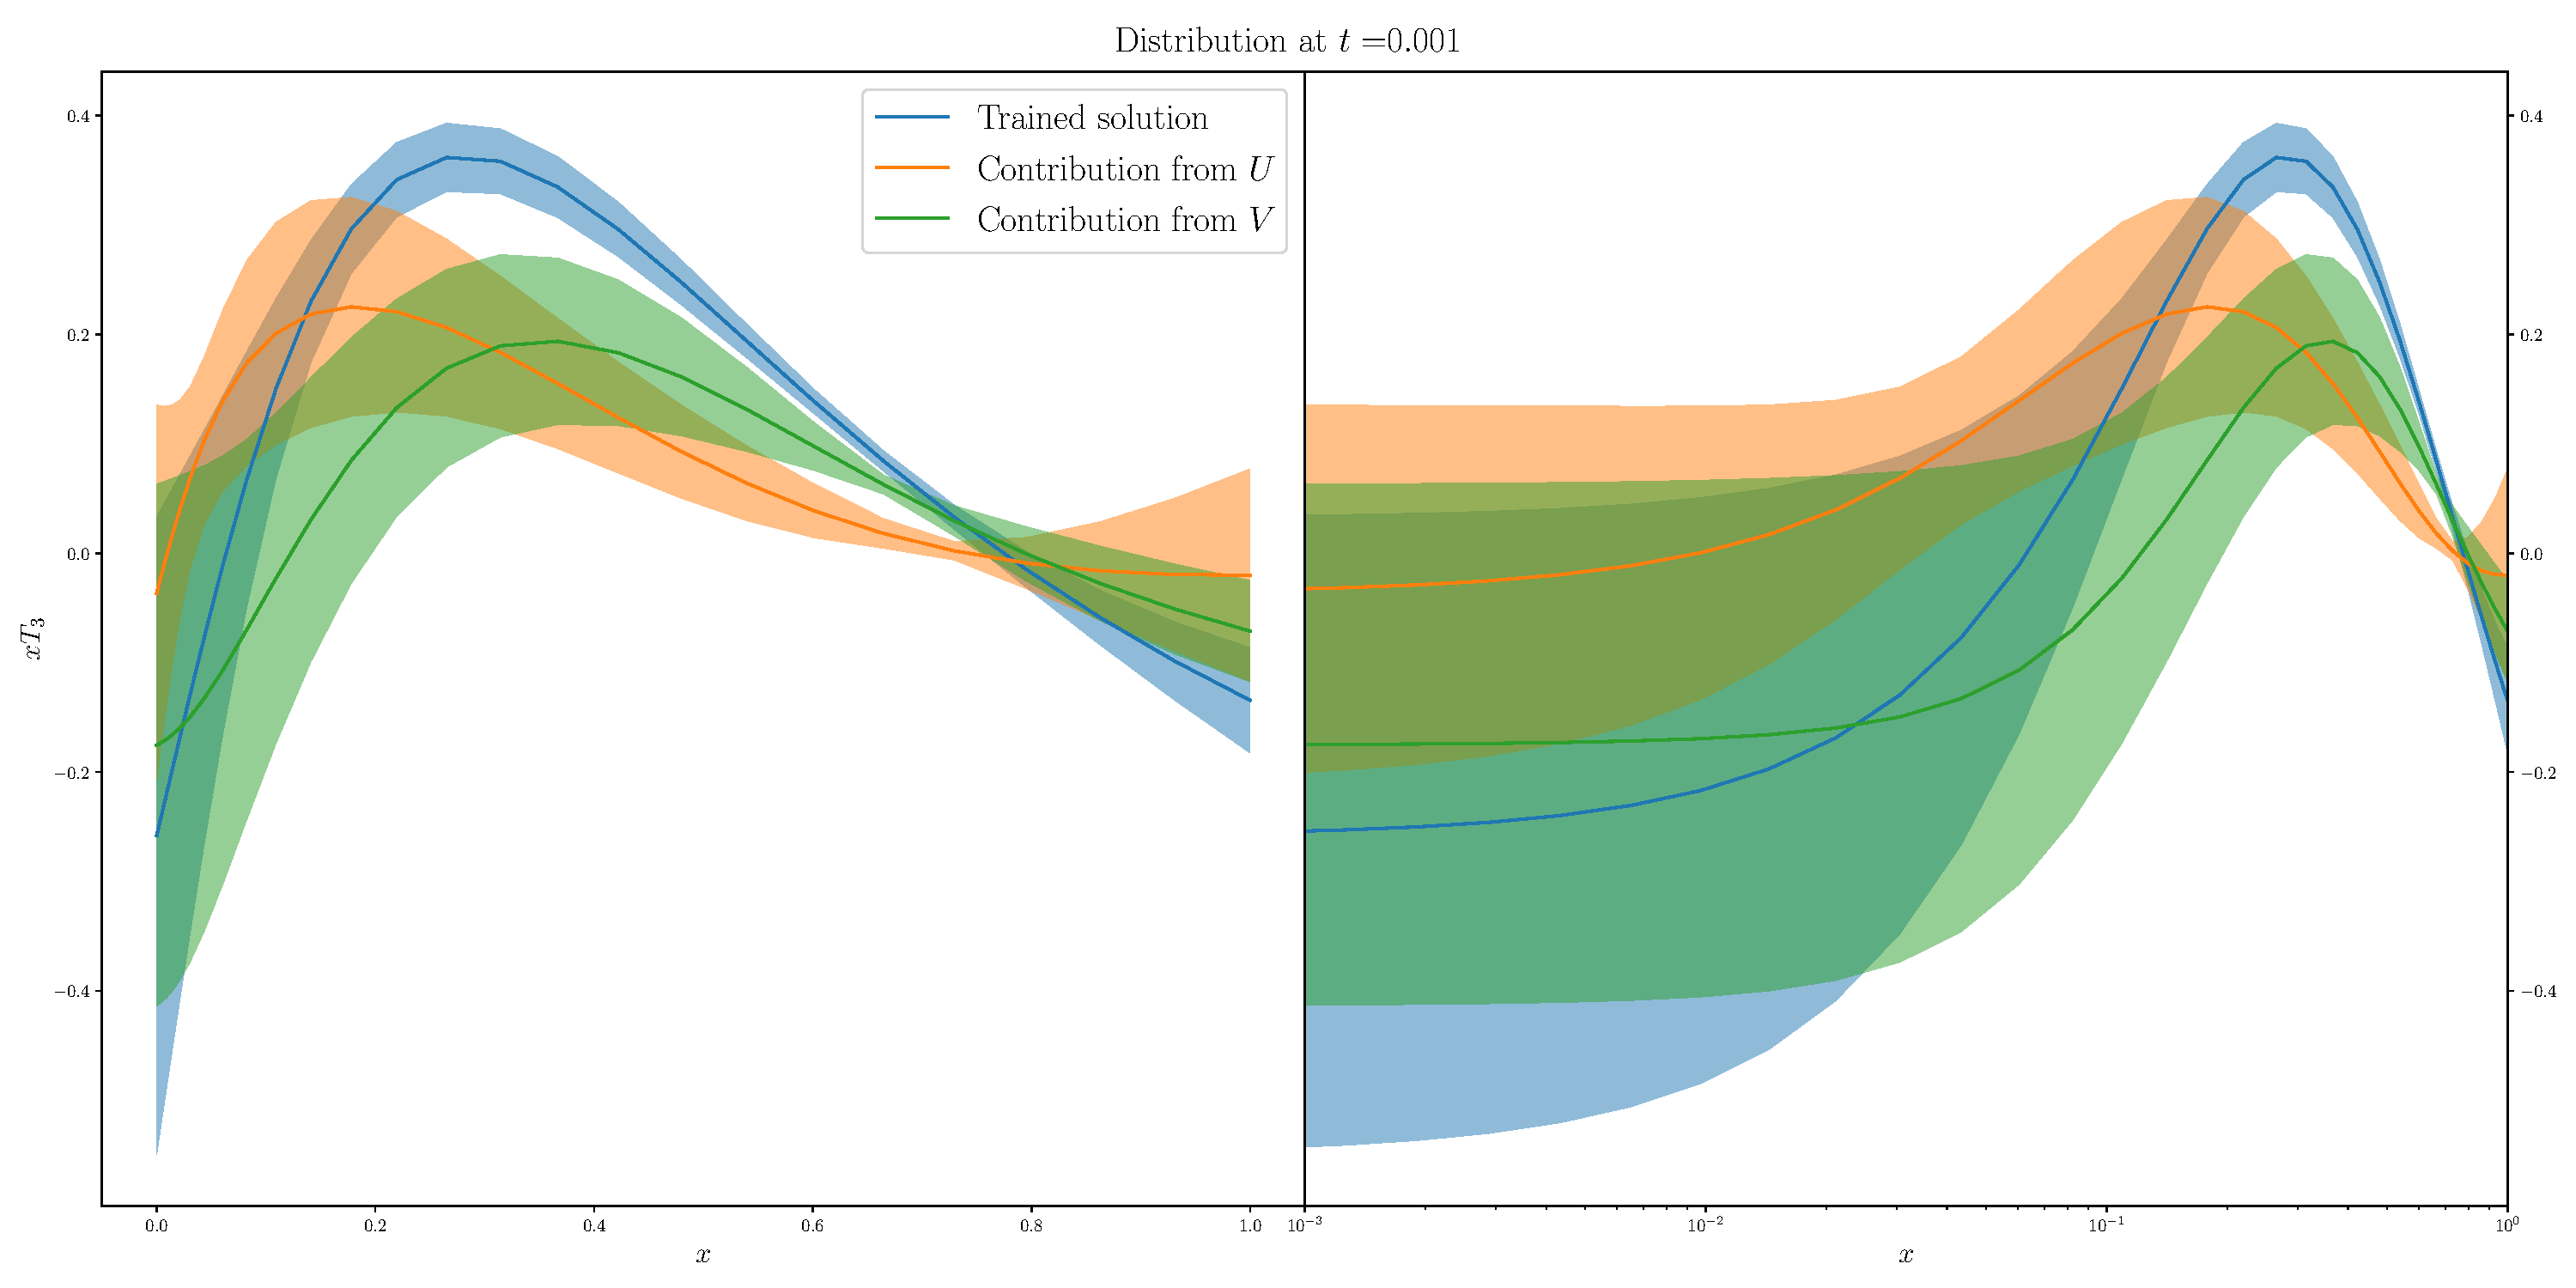
\includegraphics[width=0.65\textwidth]{plots/xT3_u_v_contribution_small_t.pdf}
  \\
  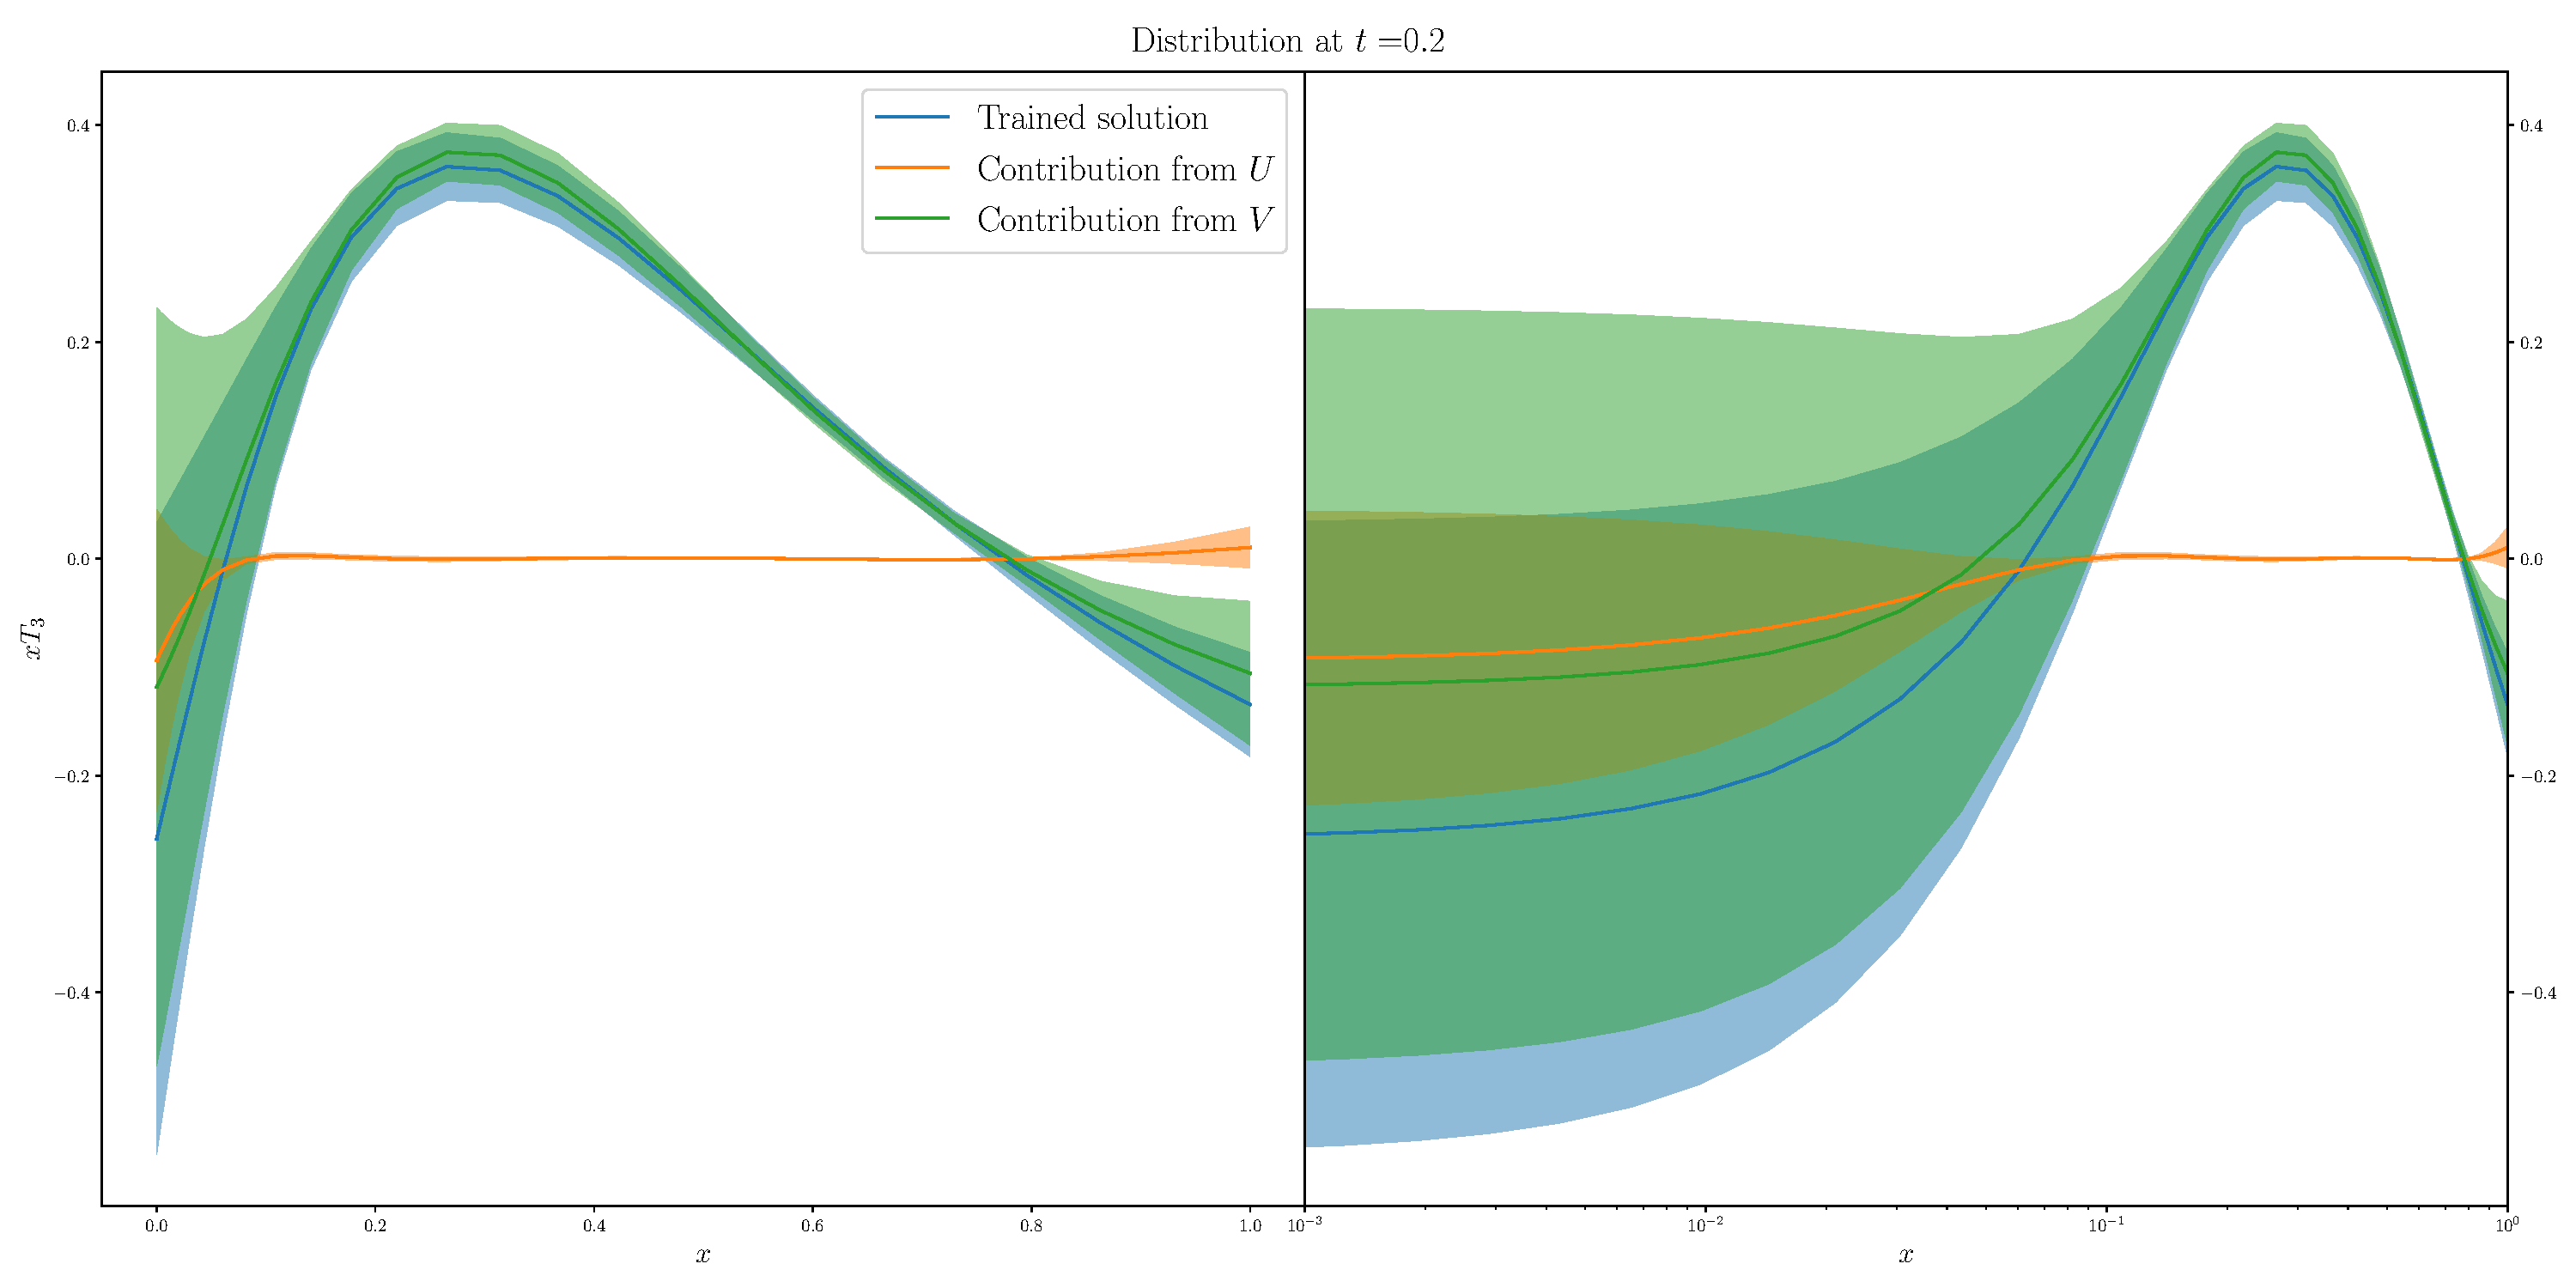
\includegraphics[width=0.65\textwidth]{plots/xT3_u_v_contribution_eot.pdf}
  \caption{Contribution of the $U$ and $V$ terms to the solution. The top panel
  shows this breakdown at early stages of the analytical training ($t=0.001$);
  the bottom panel shows the contributions at the end of training (eot) (same as
  Fig.~\ref{fig:xT3_analytical}). These plots have been obtained by taking the
  $t_{\rm ref} = 30000$ and $f_0 = f_{t_{\rm ref}}$ using L2 data. \ac{These
  plots will be modified (font size, etc...) to match the other figures.}}
\end{figure}
% ===================================

\begin{figure}[t!]
  \centering
  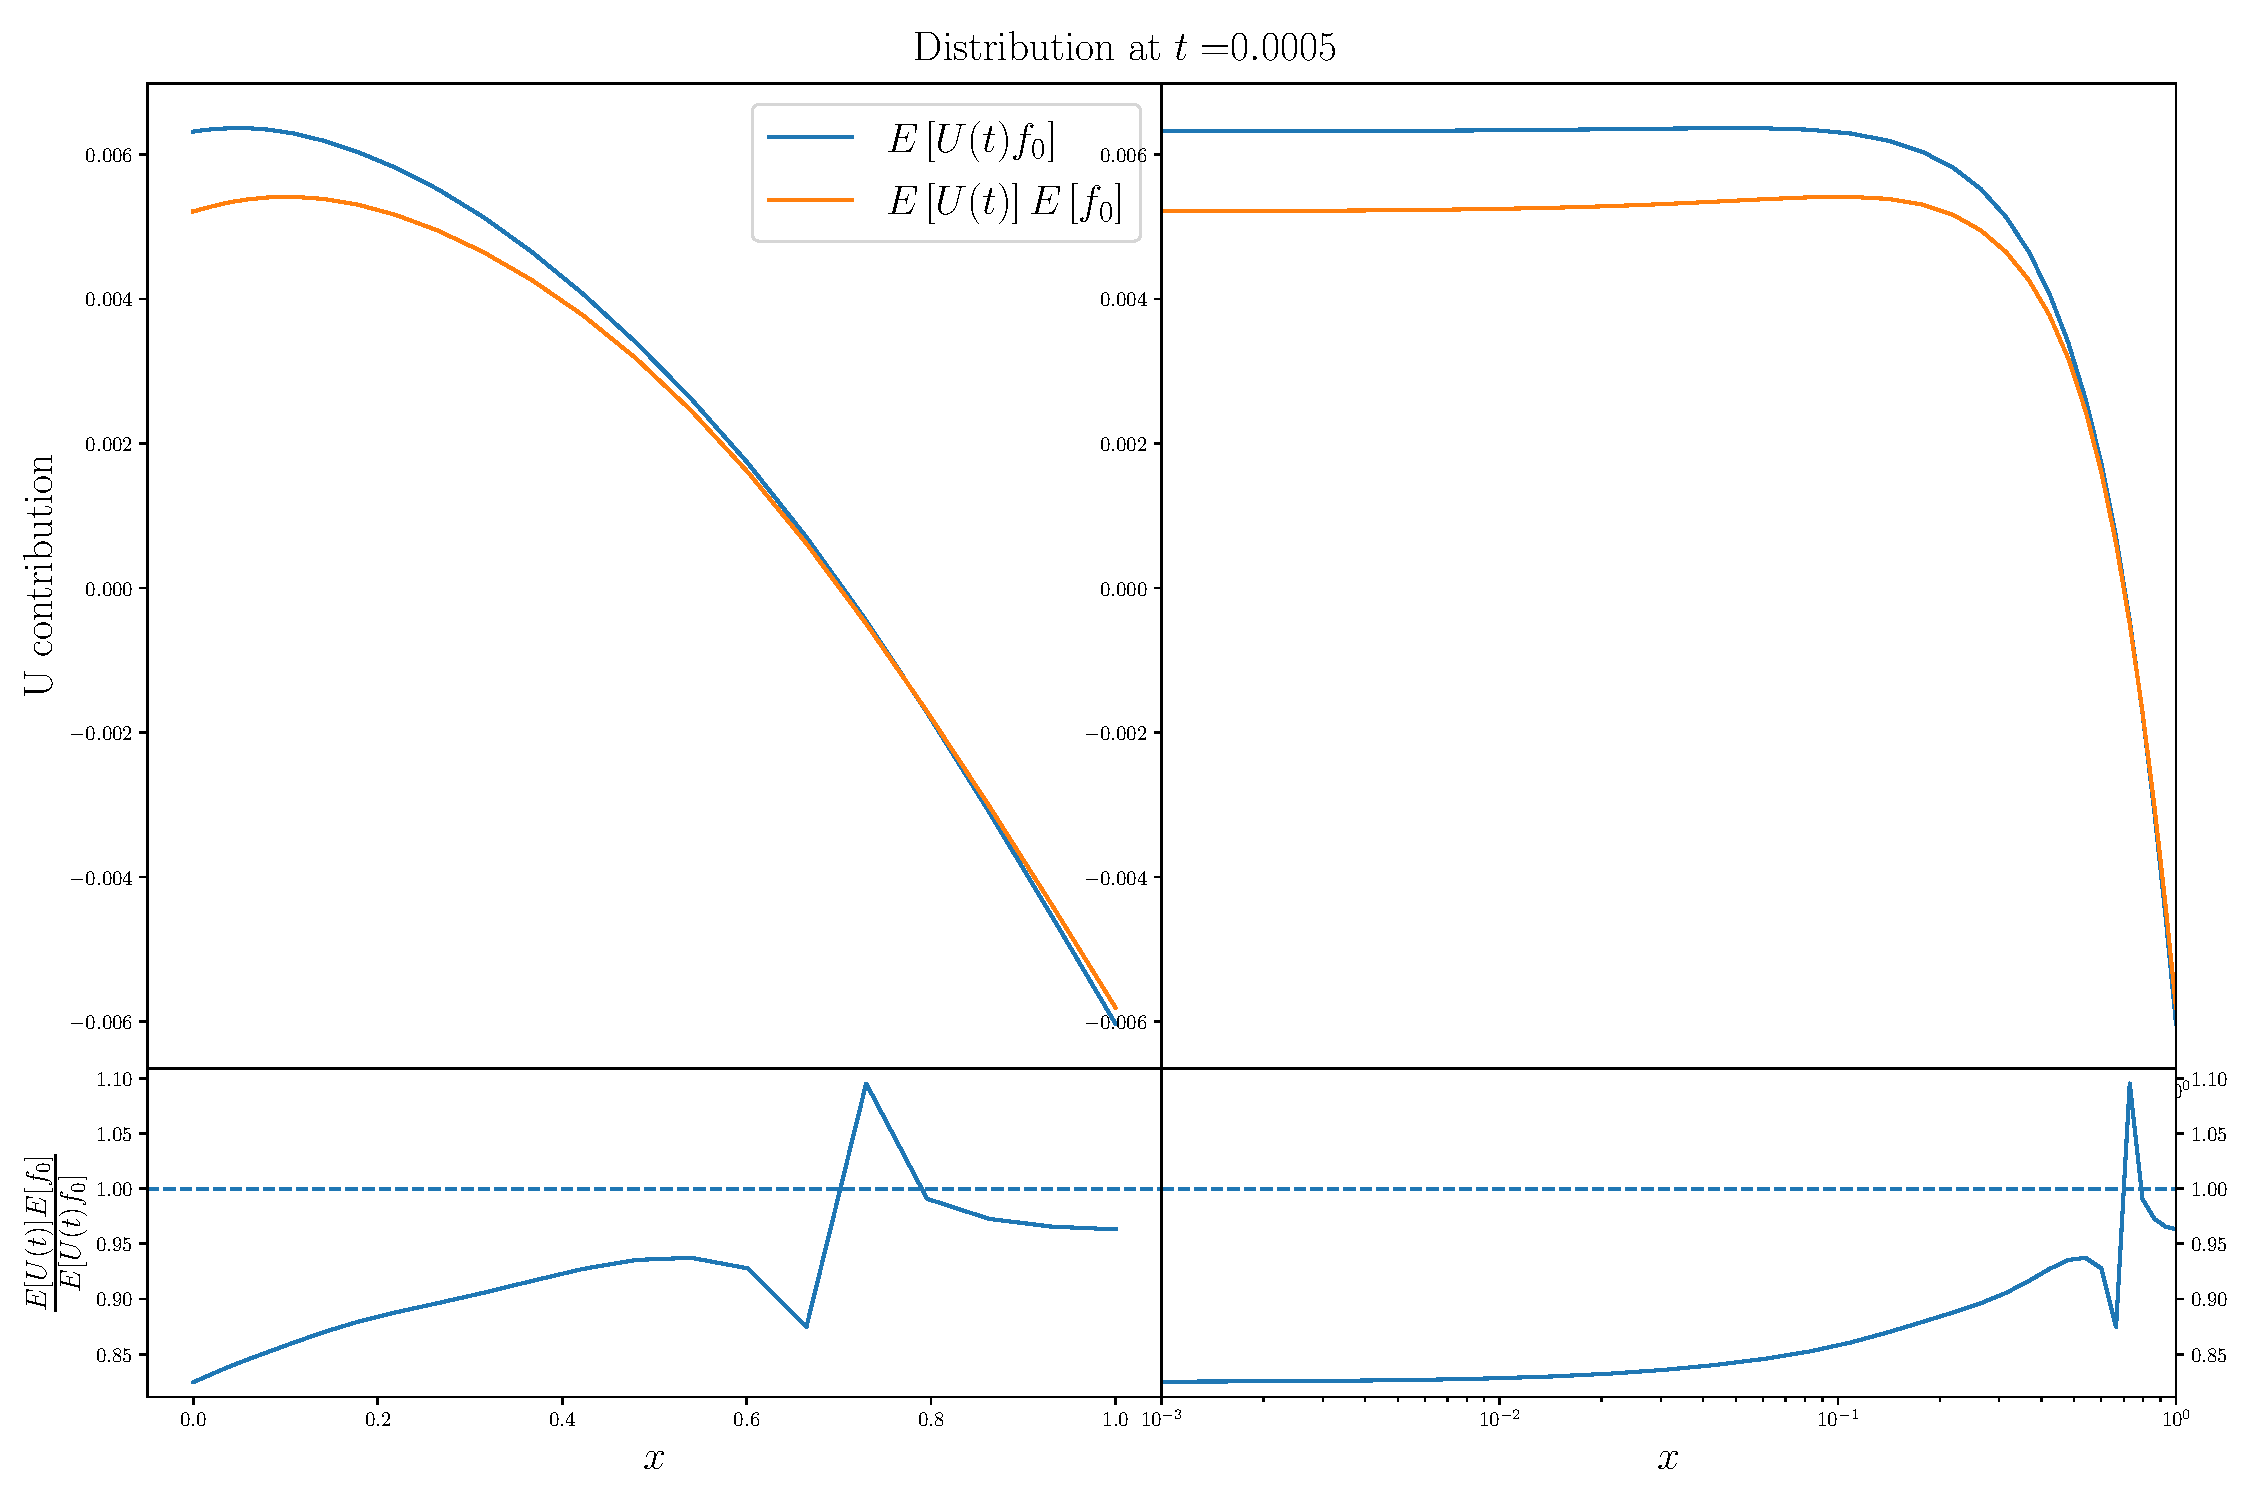
\includegraphics[width=0.65\textwidth]{plots/xT3_exp_val_early.pdf} \\
  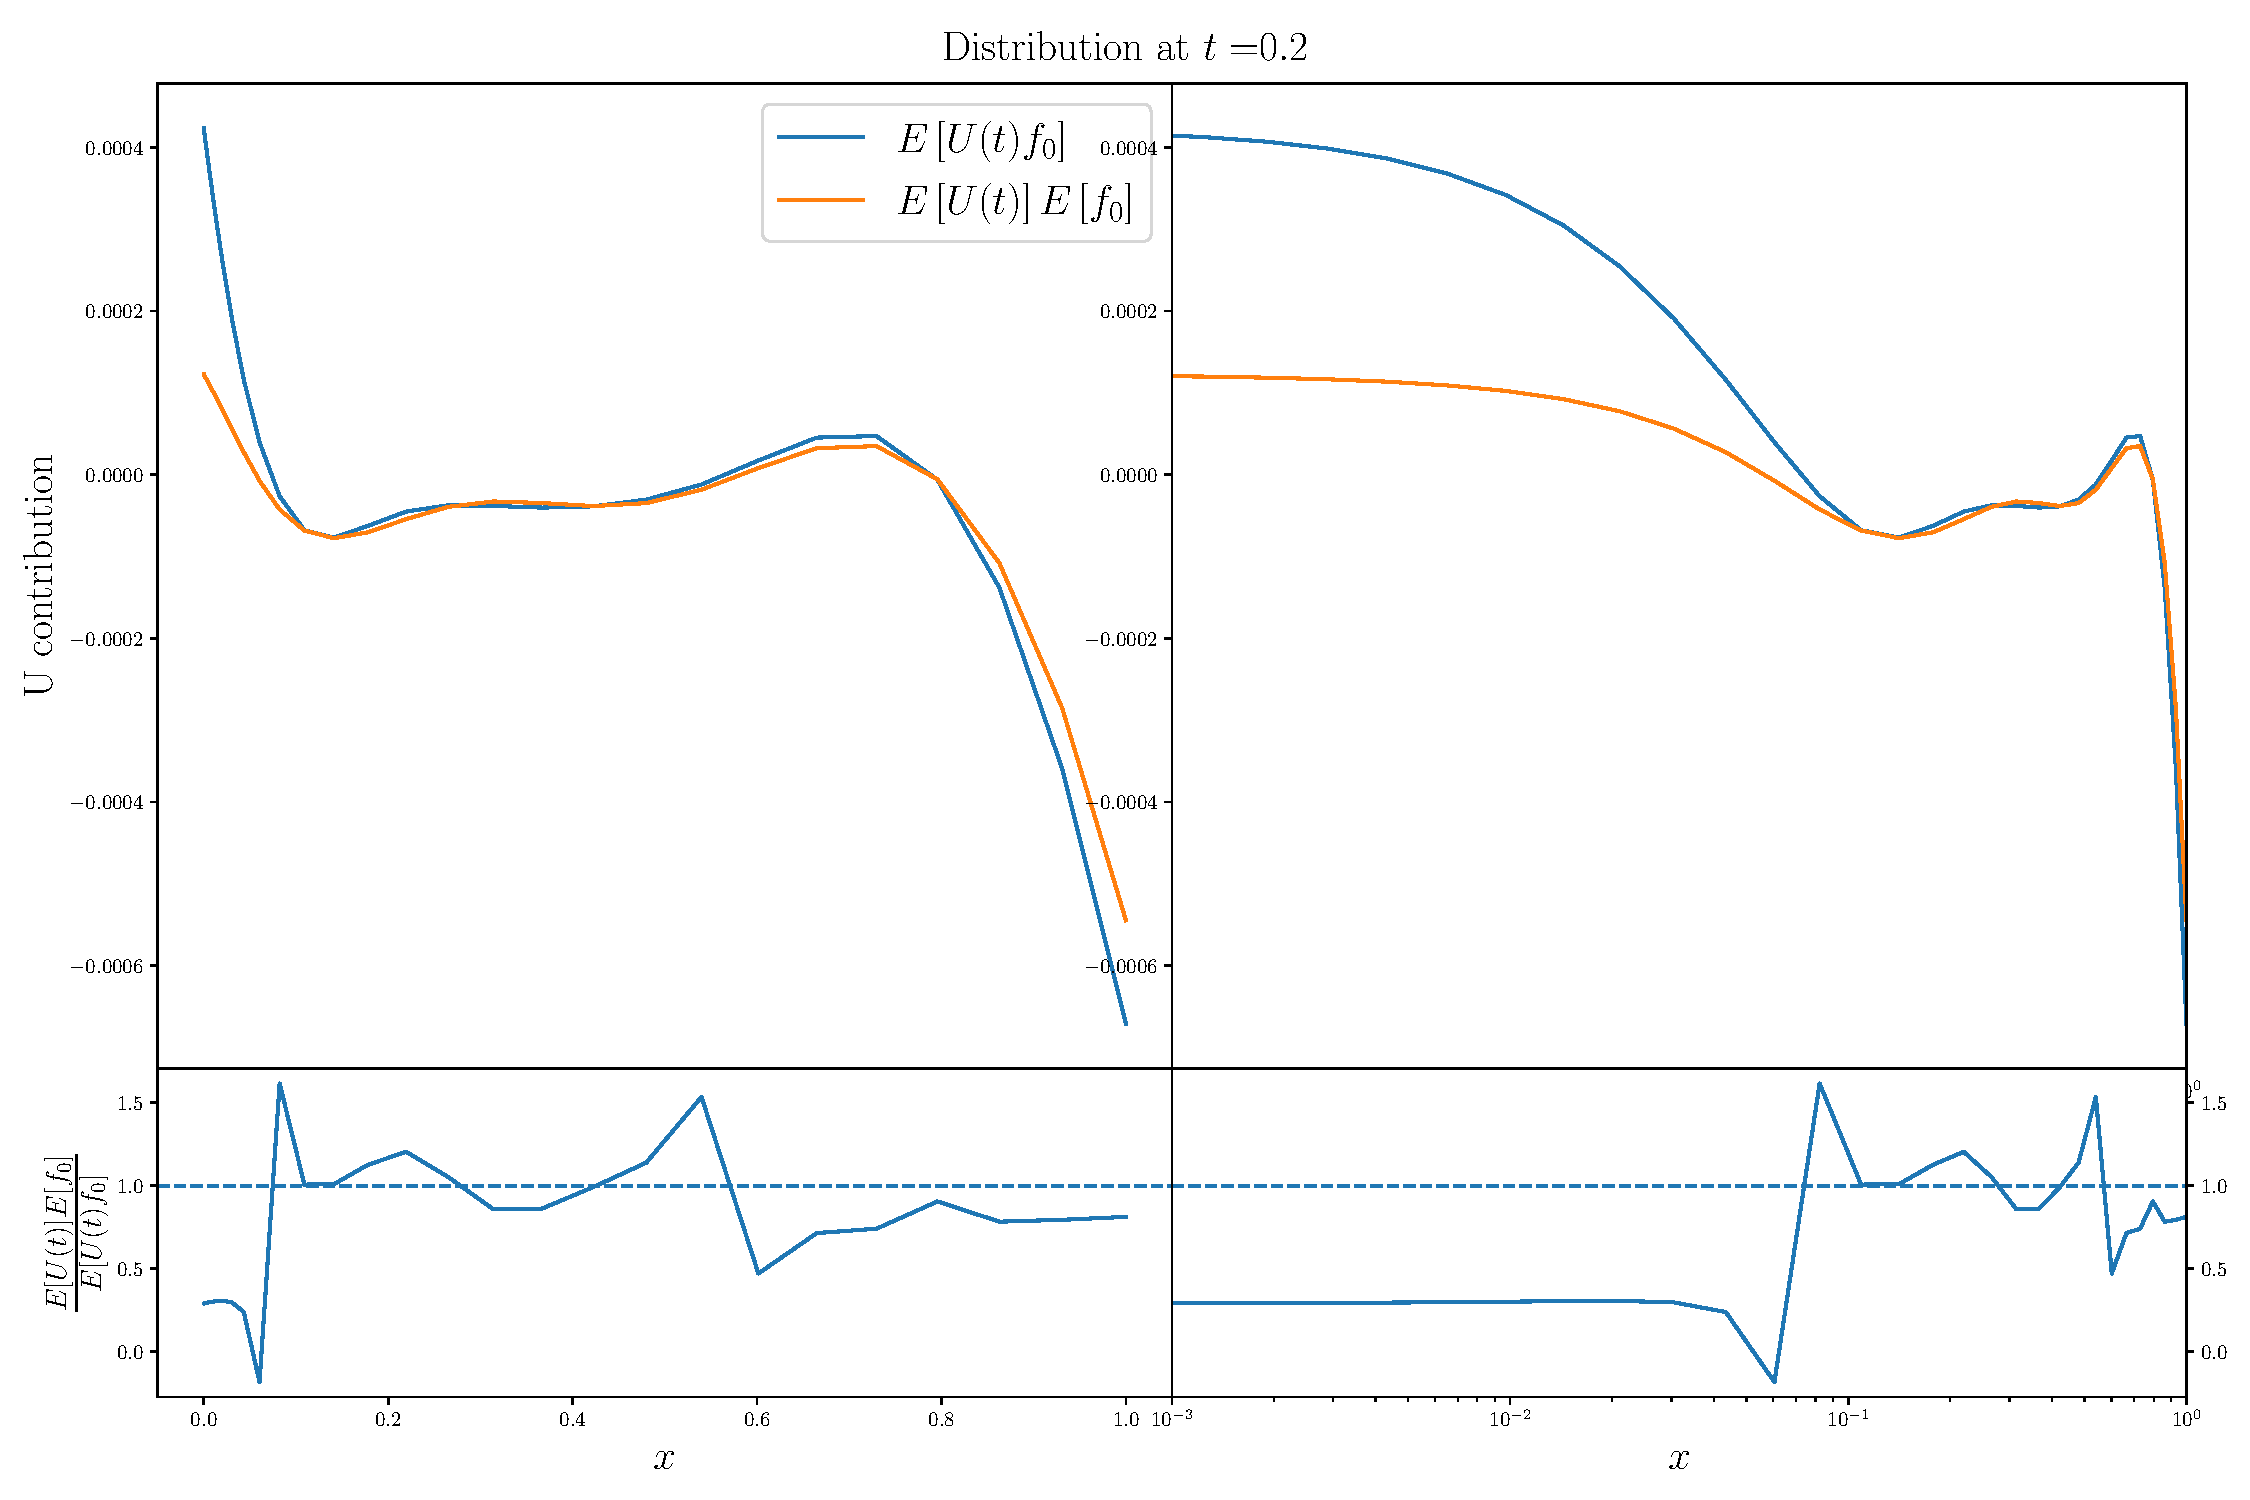
\includegraphics[width=0.65\textwidth]{plots/xT3_exp_val_eot.pdf}
  \caption{Expectation value of the product (blue) and product of the
  expectation value for the $U$ contribution. Plots obtained using $t_{\rm ref}
  = 30000$, while $f_0$ is an ensemble of networks at initialisation
  (\textit{i.e.} $\mathbb{E}[f_0]=0$). \ac{These plots will be modified (font
  size, etc...) to match the other figures.}}
\end{figure}
% ===================================


% L0 data
\begin{figure}[ht!]
    \centering
    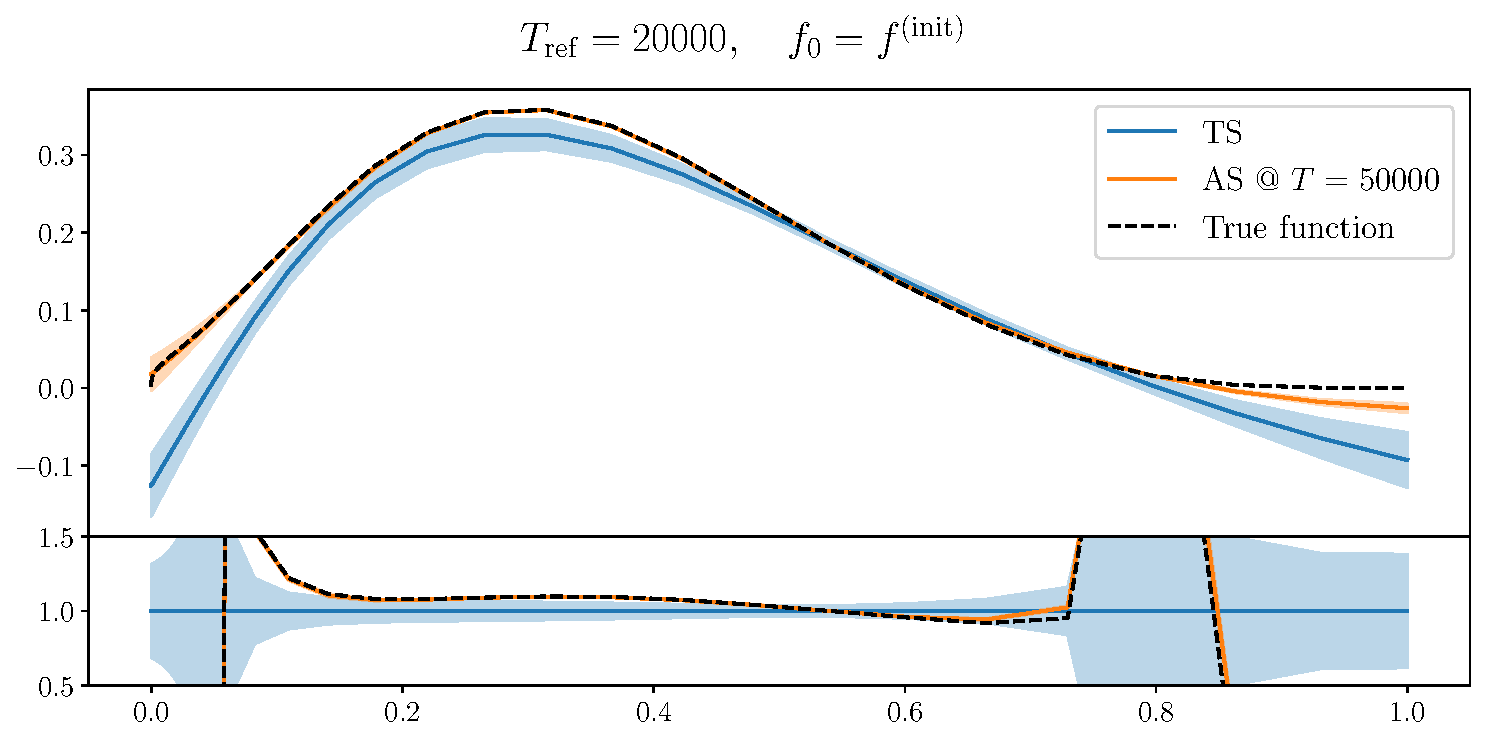
\includegraphics[width=0.48\textwidth]{plots/analytical_solution/pdf_plot_init_last_epoch_L0.pdf}
    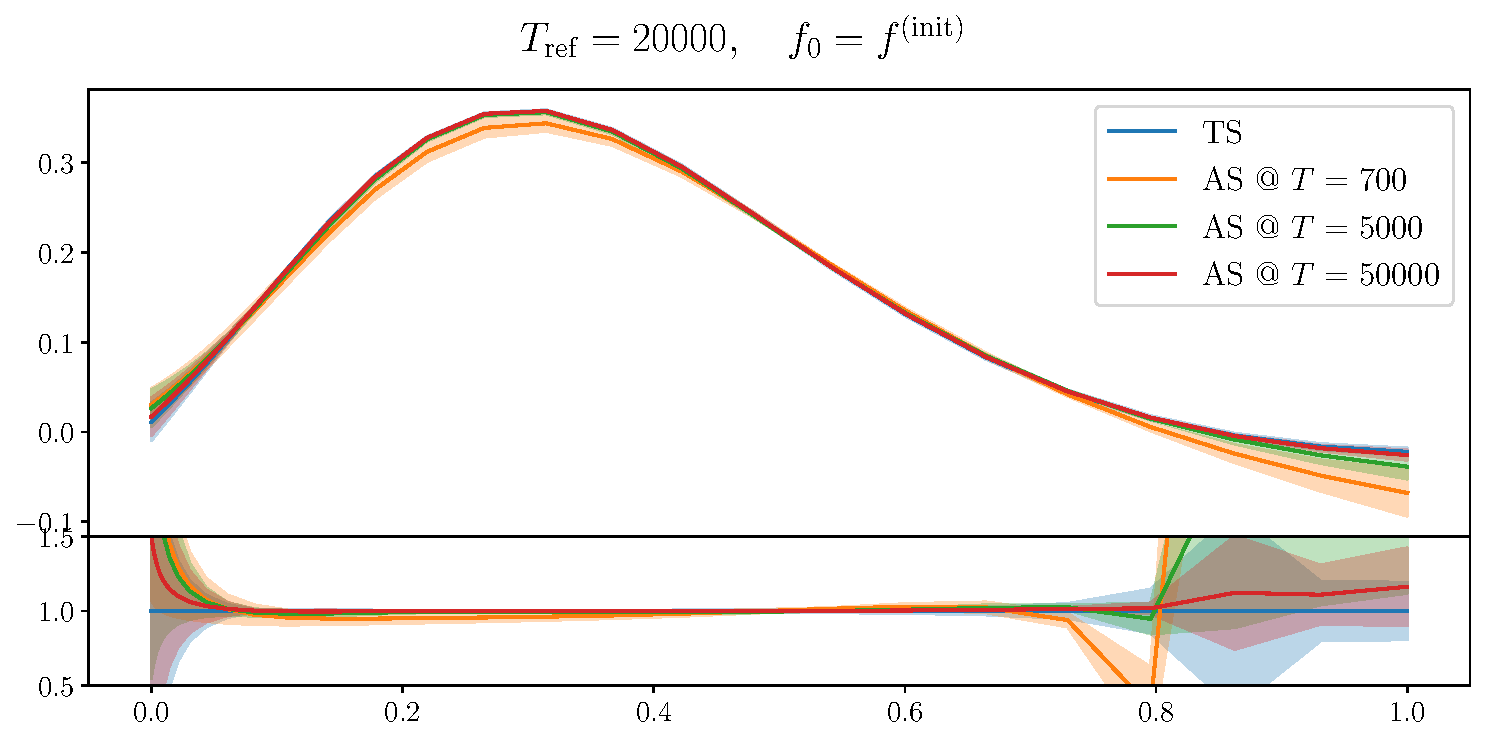
\includegraphics[width=0.48\textwidth]{plots/analytical_solution/pdf_plot_init_epochs_L0.pdf}
    \caption{Comparison of the trained solution at the end of training and
    the analytical solution using L0 data. In both panels, the
    frozen NTK is chosen at $T_{\rm ref} = 20000$ and the initial function $f_0$
    is a different ensemble of networks at initialisation. In the left panel,
    the analytical solution is evolved for $T_{\rm tot}$ epochs, while the right
    panel shows the same comparison for intermediate epochs.}
    \label{fig:xT3_analytical_init_L0}
  \end{figure}
  % ===================================
  \begin{figure}[ht!]
    \centering
    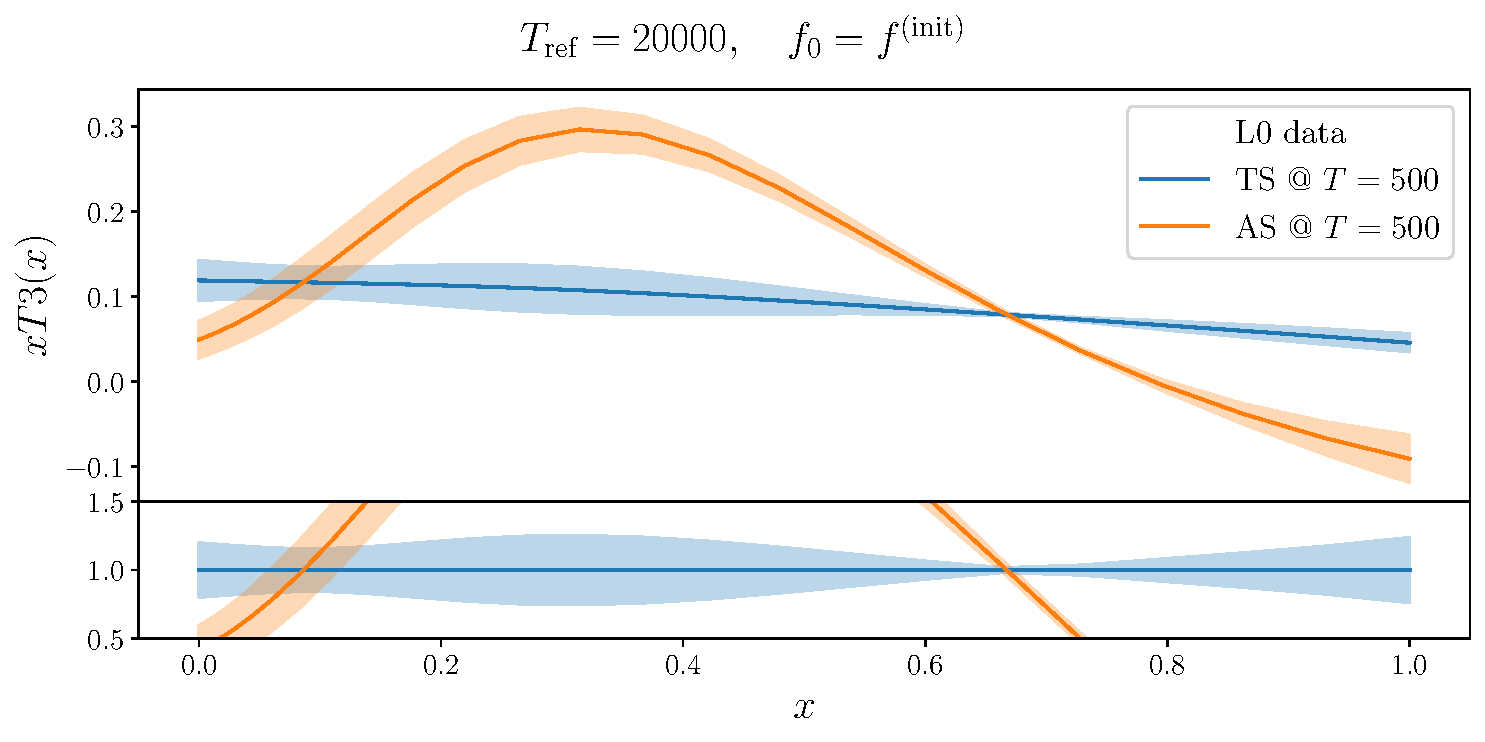
\includegraphics[width=0.45\textwidth]{plots/analytical_solution/evolution_vs_trained_epoch_500_L0.pdf} \hspace{10mm}
    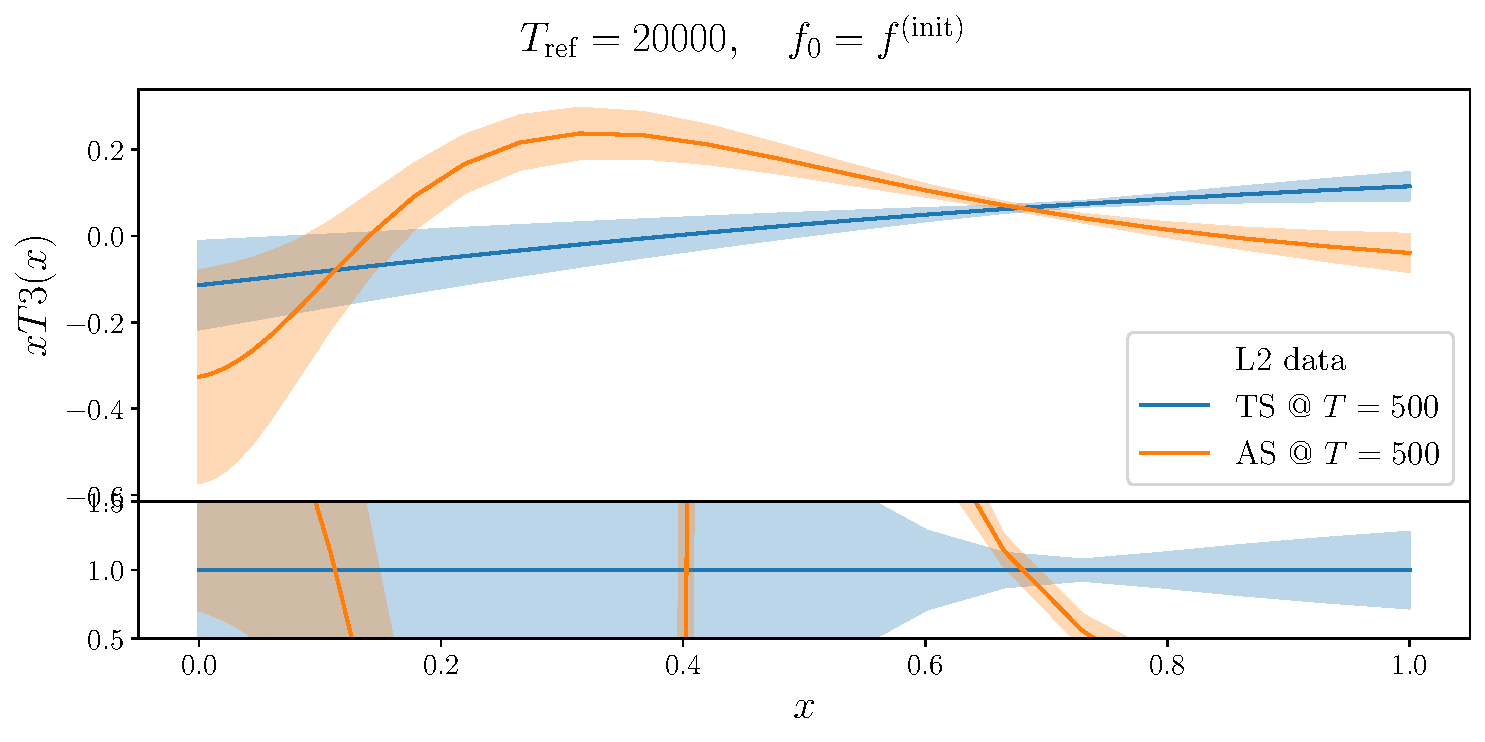
\includegraphics[width=0.45\textwidth]{plots/analytical_solution/evolution_vs_trained_epoch_500_L2.pdf}
    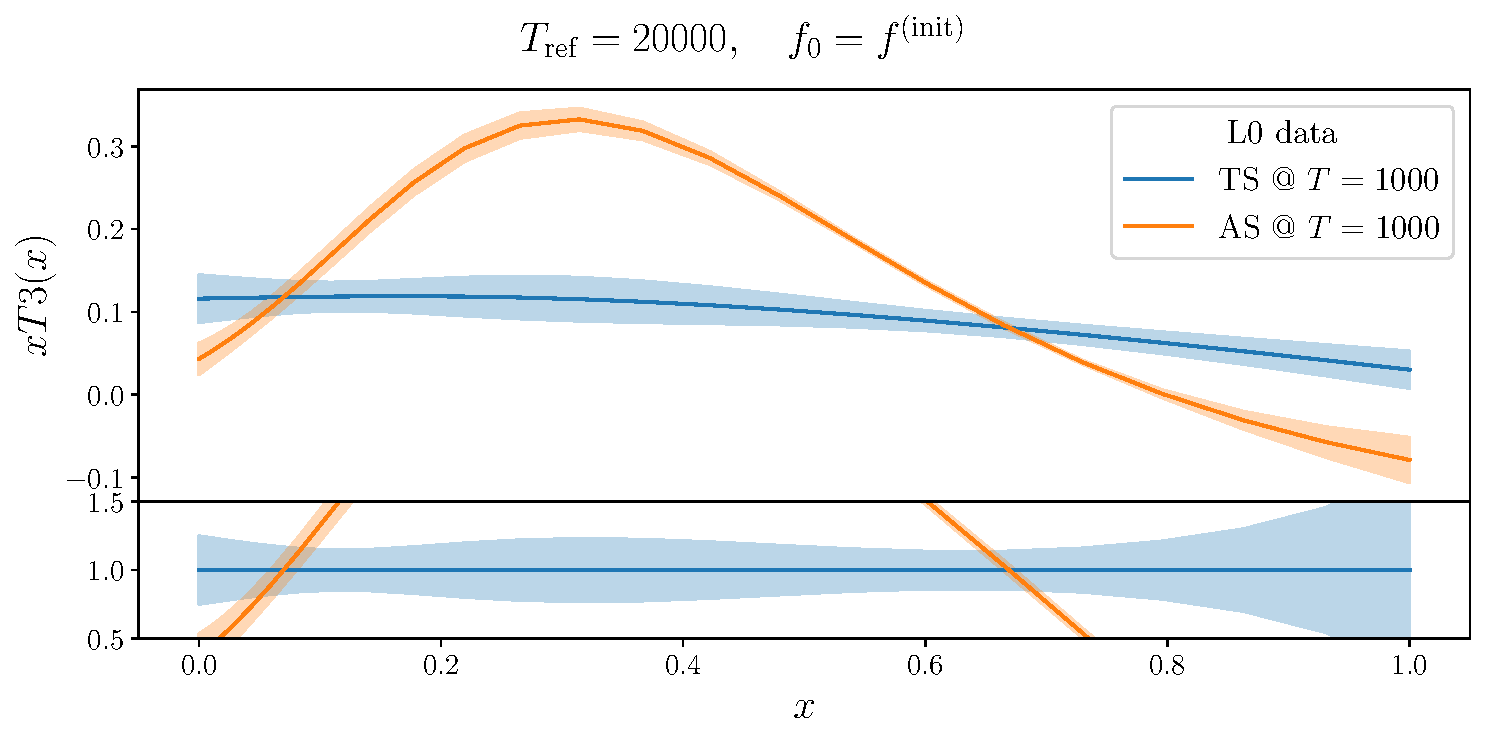
\includegraphics[width=0.45\textwidth]{plots/analytical_solution/evolution_vs_trained_epoch_1000_L0.pdf} \hspace{10mm}
    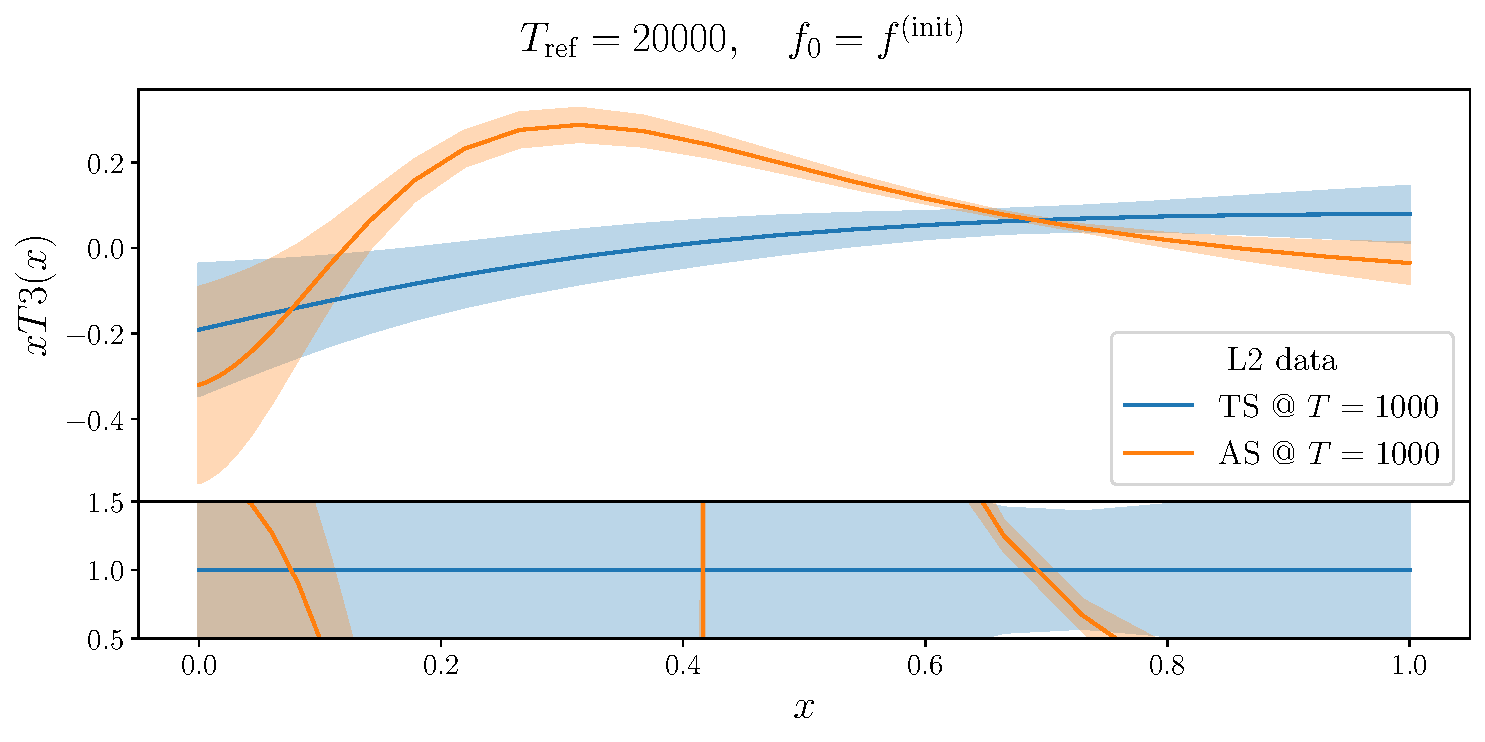
\includegraphics[width=0.45\textwidth]{plots/analytical_solution/evolution_vs_trained_epoch_1000_L2.pdf}
    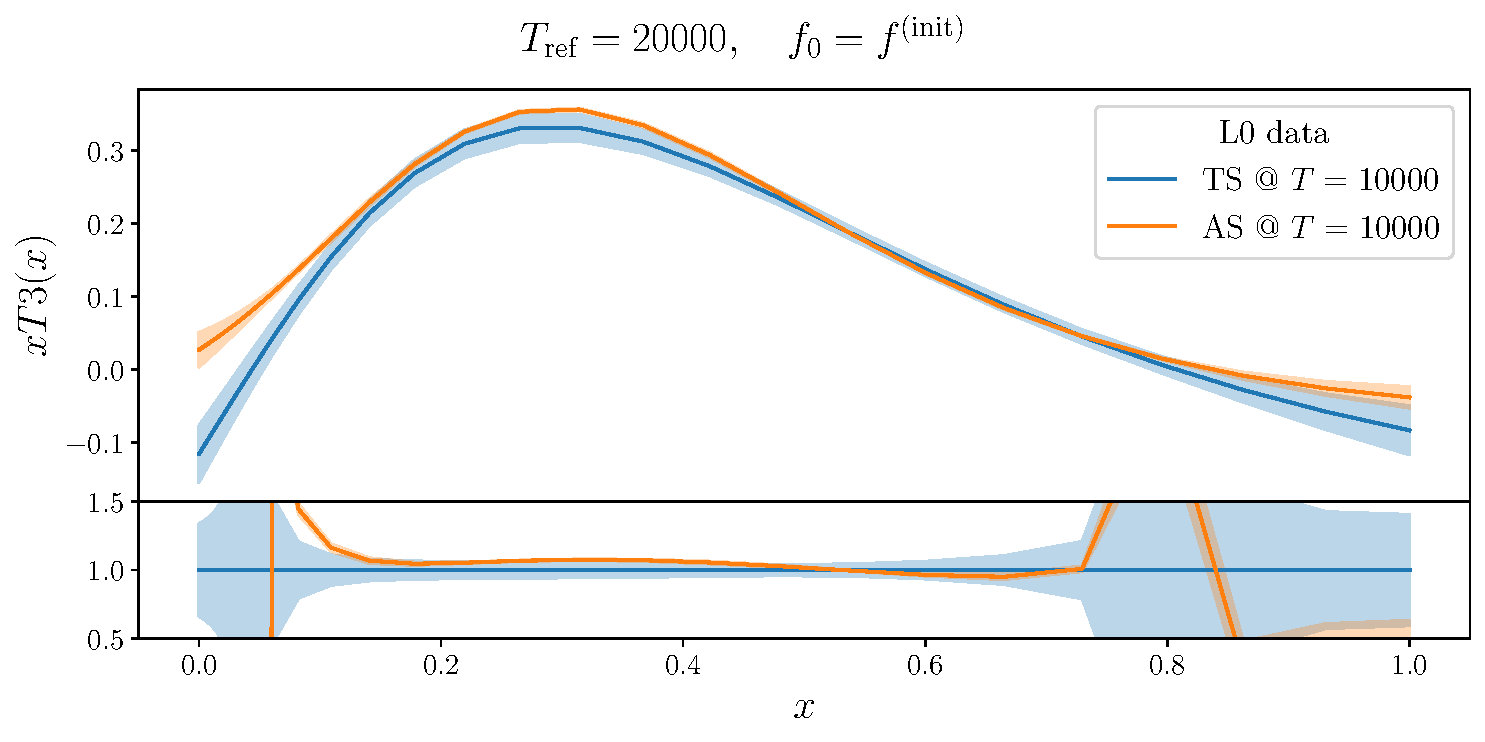
\includegraphics[width=0.45\textwidth]{plots/analytical_solution/evolution_vs_trained_epoch_10000_L0.pdf} \hspace{10mm}
    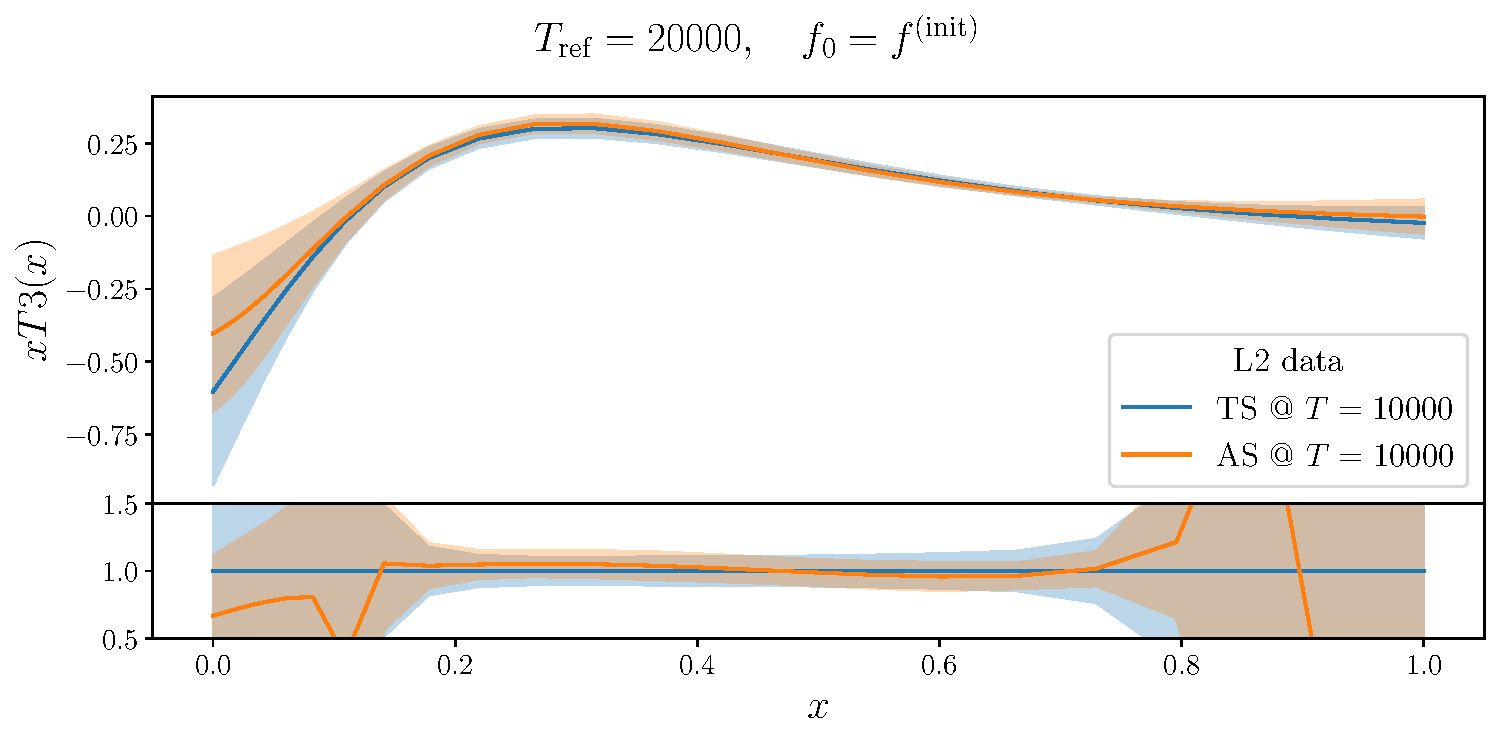
\includegraphics[width=0.45\textwidth]{plots/analytical_solution/evolution_vs_trained_epoch_10000_L2.pdf}
    \caption{Comparison of the analytical solution and the trained solution at
    different epochs. The analytical solution is computed using the frozen NTK
    at $T_{\rm ref} = 20000$ and the initial function $f_0$ is a different
    ensemble of networks at initialisation. Left column shows results for L0
    data, while the right column shows results for L2 data.}
    \label{fig:xT3_analytical_vs_trained}
  \end{figure}
  % ===================================
  \begin{figure}[ht!]
    \centering
    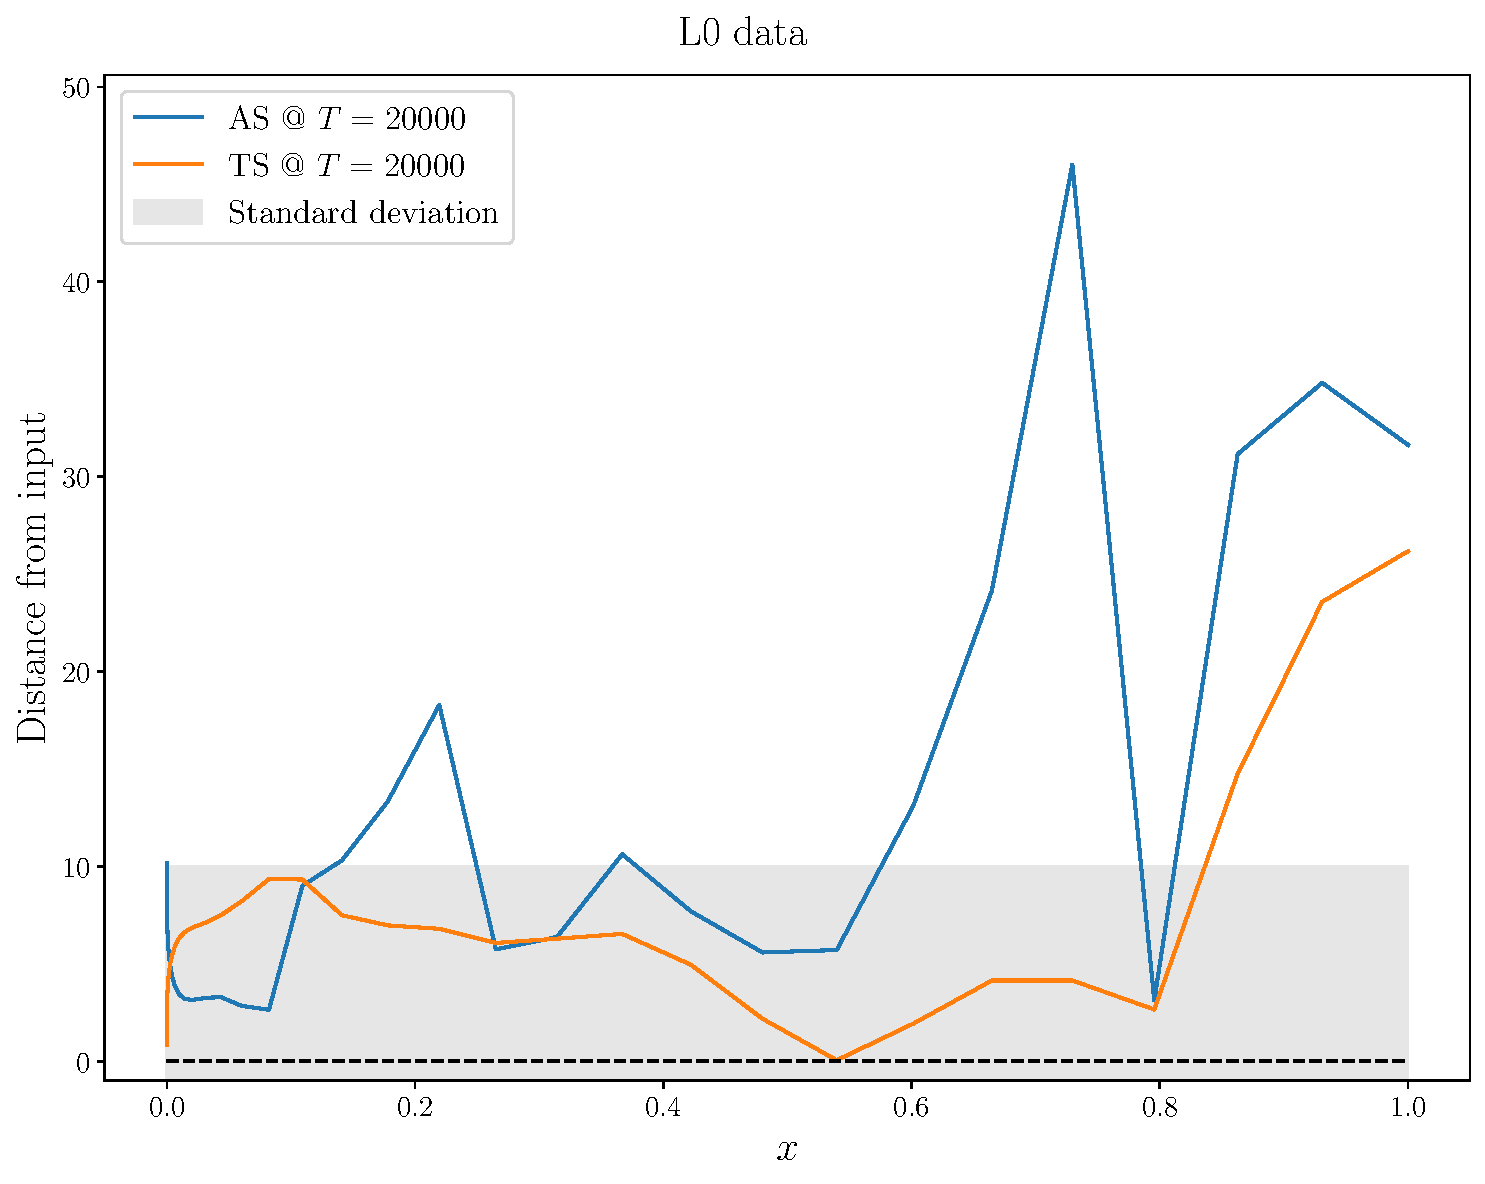
\includegraphics[width=0.48\textwidth]{plots/analytical_solution/distance_plot_from_fin_L0.pdf}
    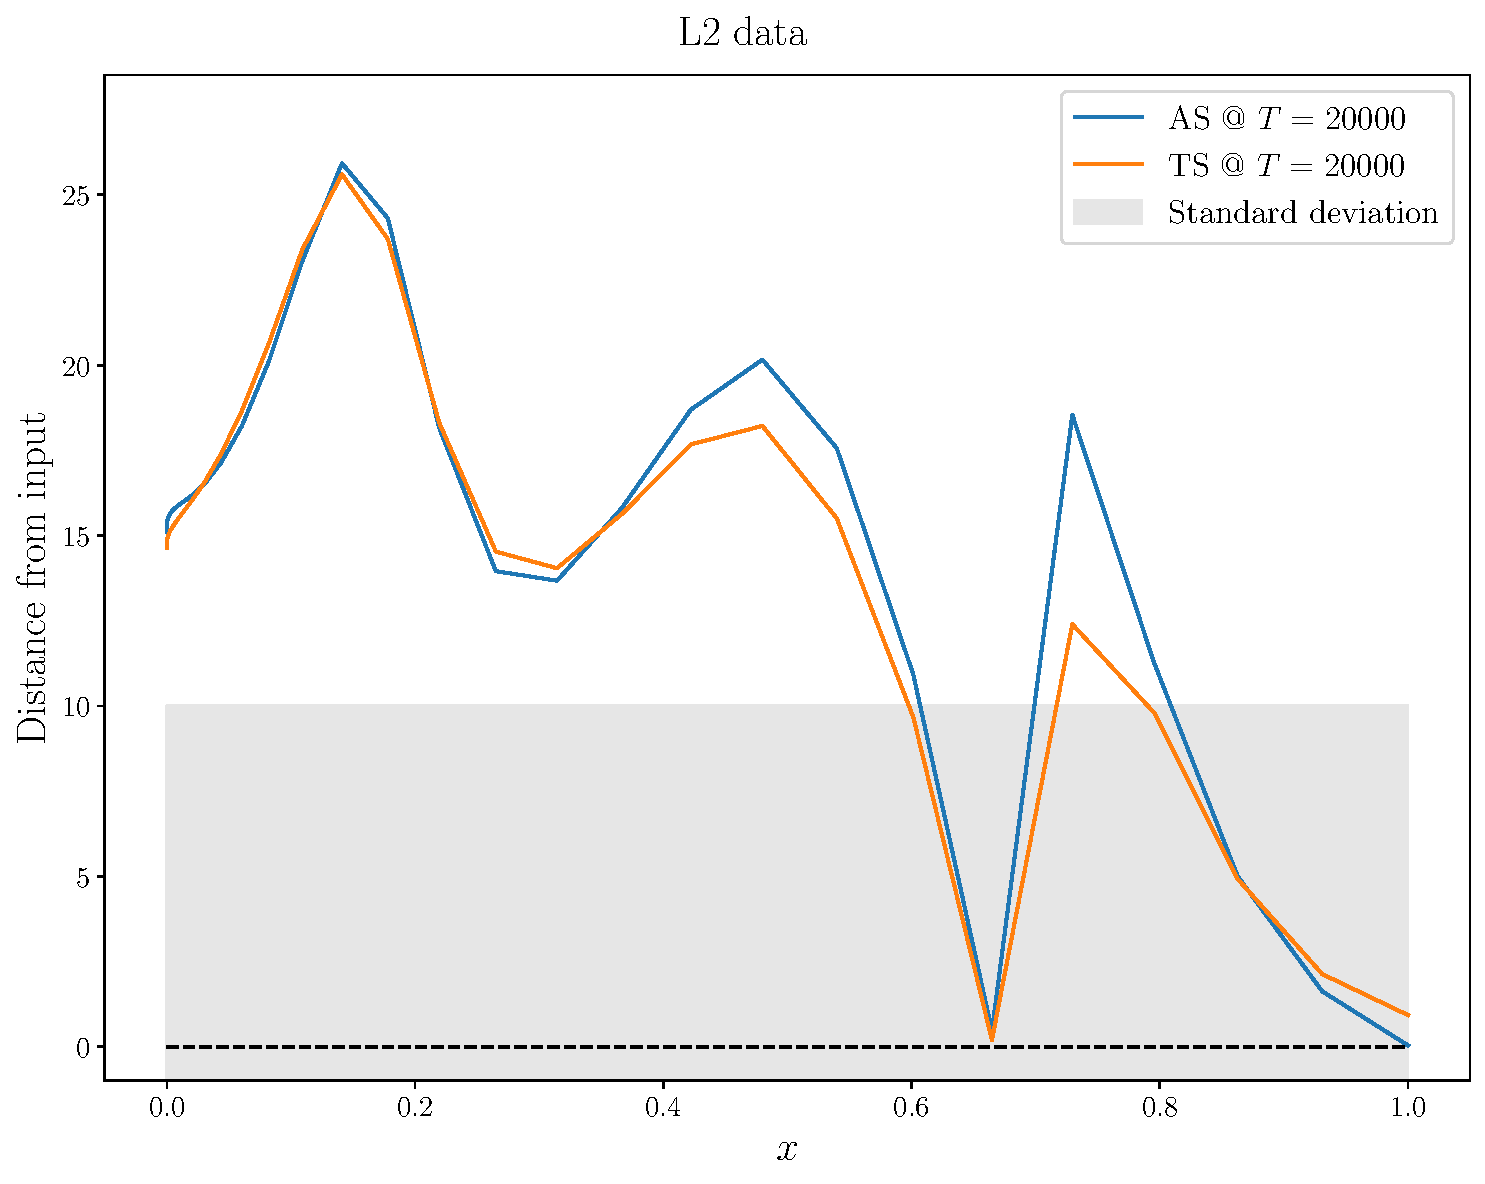
\includegraphics[width=0.48\textwidth]{plots/analytical_solution/distance_plot_from_fin_L2.pdf}
    \caption{PDF distance, as defined in Ref.~\cite{NNPDF:2021njg}, with respect to
    the input function $f^{(in)}$ used to generate the data and the analytical and trained
    solutions in function of the evaluation epochs. The frozen NTK
    is chosen at $T_{\rm ref} = 20000$ and the initial function $f_0$ is a different
    ensemble of networks at initialisation. The left panel shows the case for L0 data,
    while the right panel shows the case for L2 data.}
    \label{fig:xT3_distance_L0_L2}
  \end{figure}
  % ===================================

  % L2 data
\begin{figure}[ht!]
    \centering
    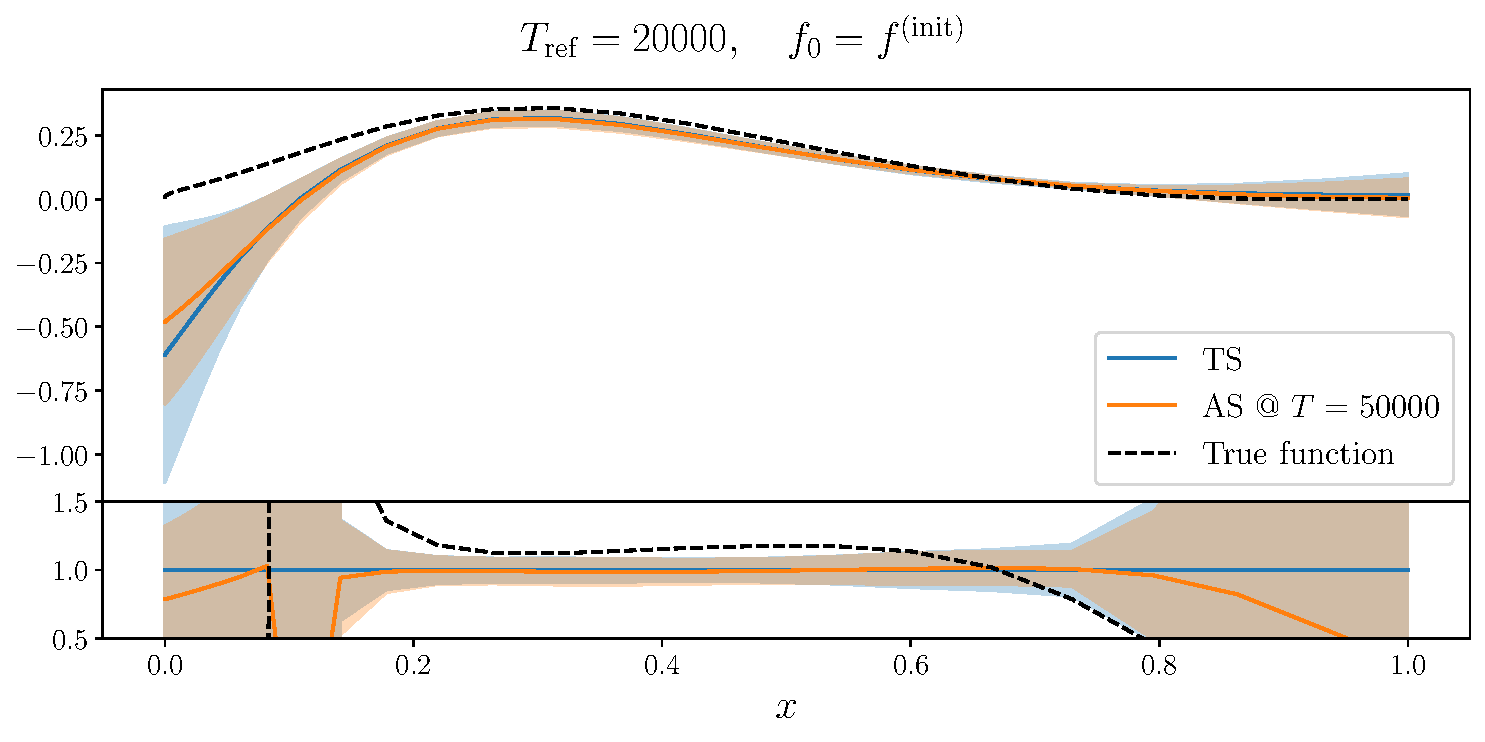
\includegraphics[width=0.48\textwidth]{plots/analytical_solution/pdf_plot_init_last_epoch_L2.pdf}
    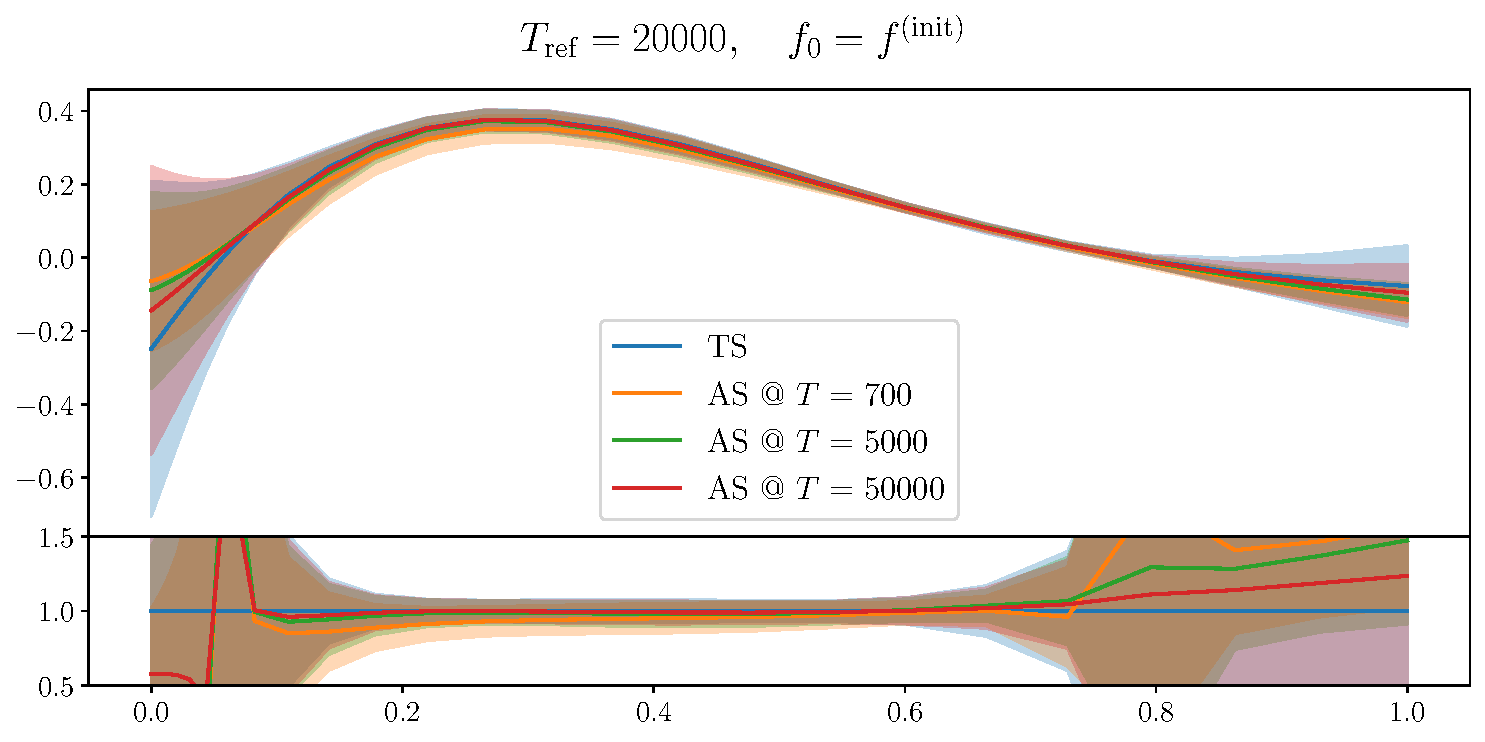
\includegraphics[width=0.48\textwidth]{plots/analytical_solution/pdf_plot_init_epochs_L2.pdf}
    \caption{Same as Fig.~\ref{fig:xT3_analytical_init_L0}, but using L2 data.}
    \label{fig:xT3_analytical_init_L2}
  \end{figure}
  % ===================================


\begin{figure}[ht!]
    \centering
    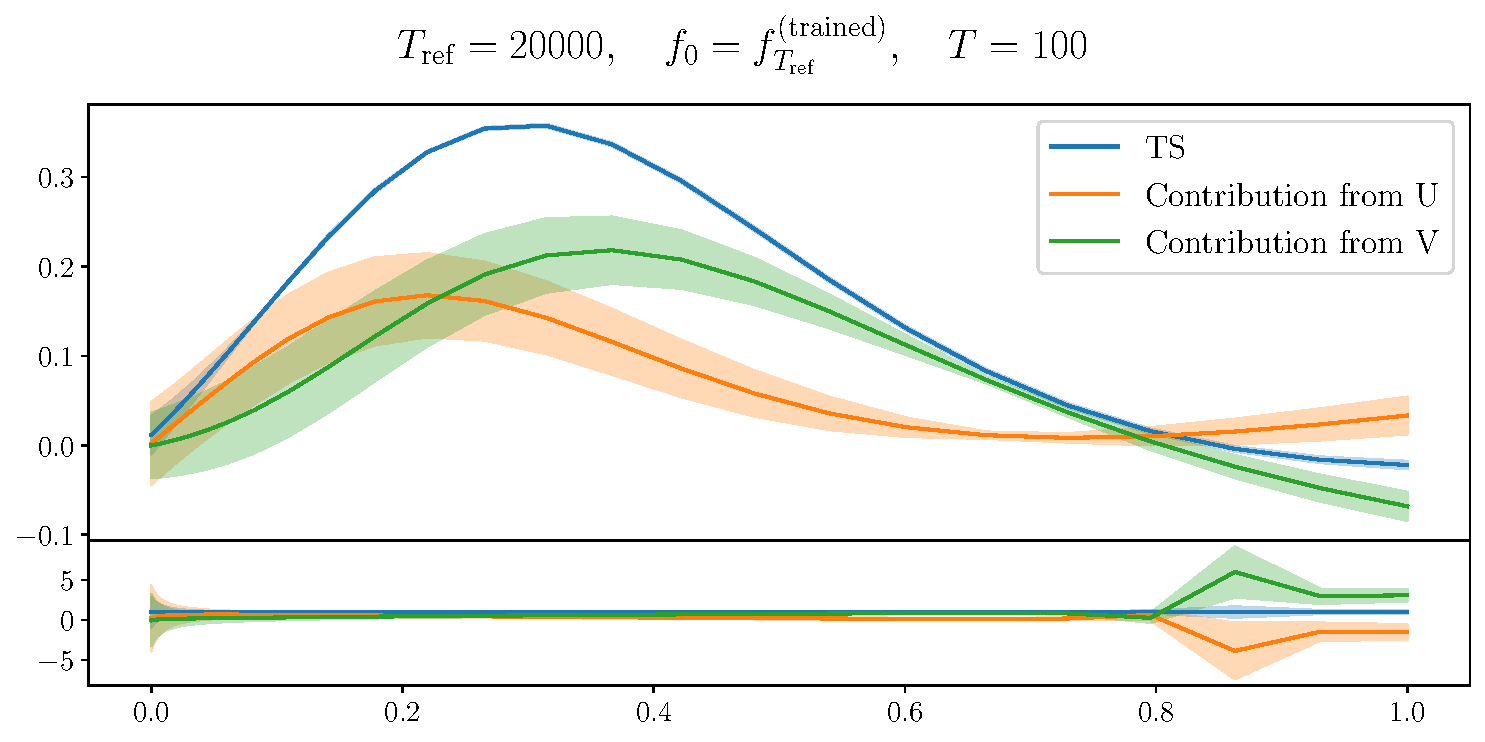
\includegraphics[width=0.45\textwidth]{plots/analytical_solution/pdf_plot_u_v_100_L0.pdf}
    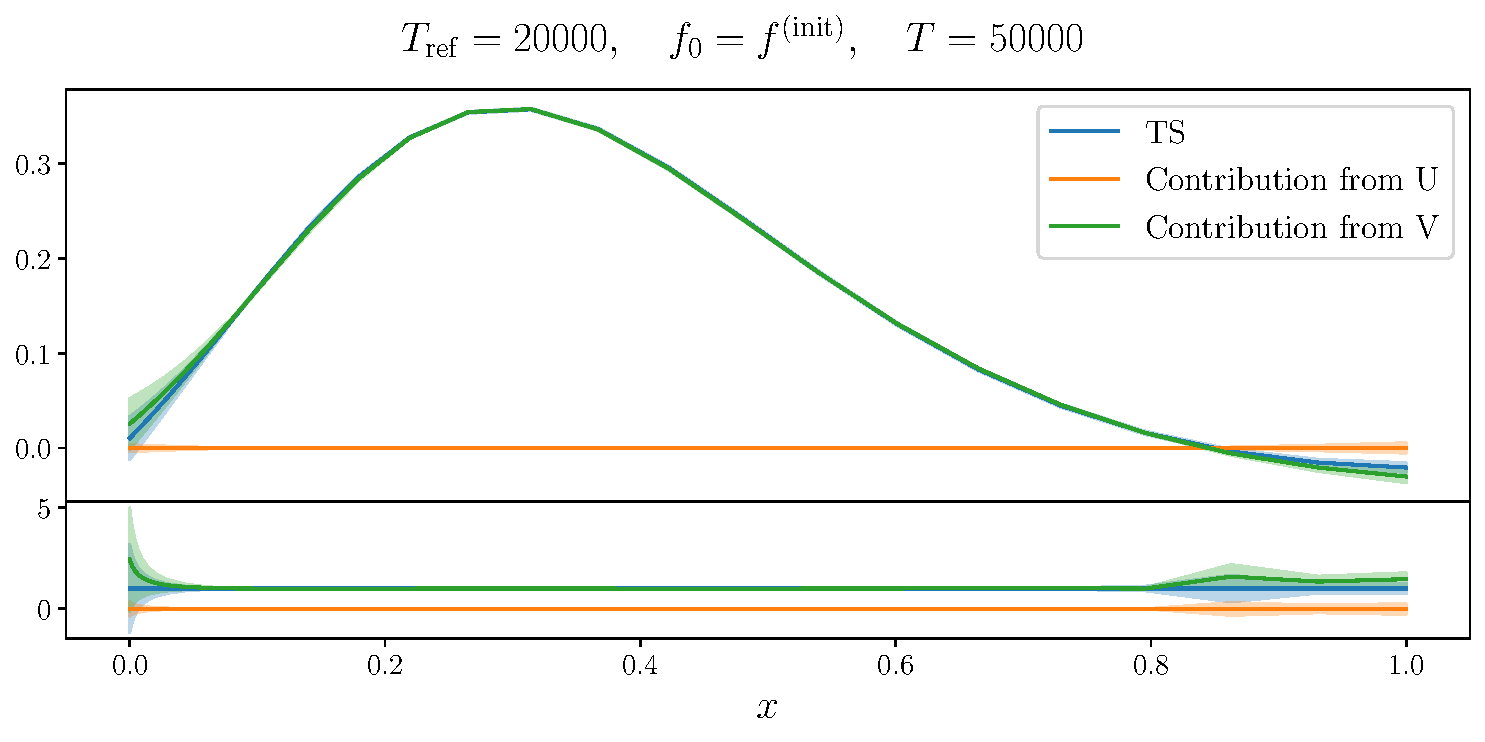
\includegraphics[width=0.45\textwidth]{plots/analytical_solution/pdf_plot_u_v_50000_L0.pdf}
    \caption{Contribution of the $U$ and $V$ terms to the analytical solution. The left
    panel shows this breakdown at early stages of the analytical training
    ($T=100$ epochs); the right panel shows the contributions at the end of
    training, as in Fig.~\ref{fig:xT3_analytical_init_L0}.}
    \label{fig:xT3_u_v_contributions_L0}
  \end{figure}
  % ===================================

  \begin{figure}[ht!]
    \centering
    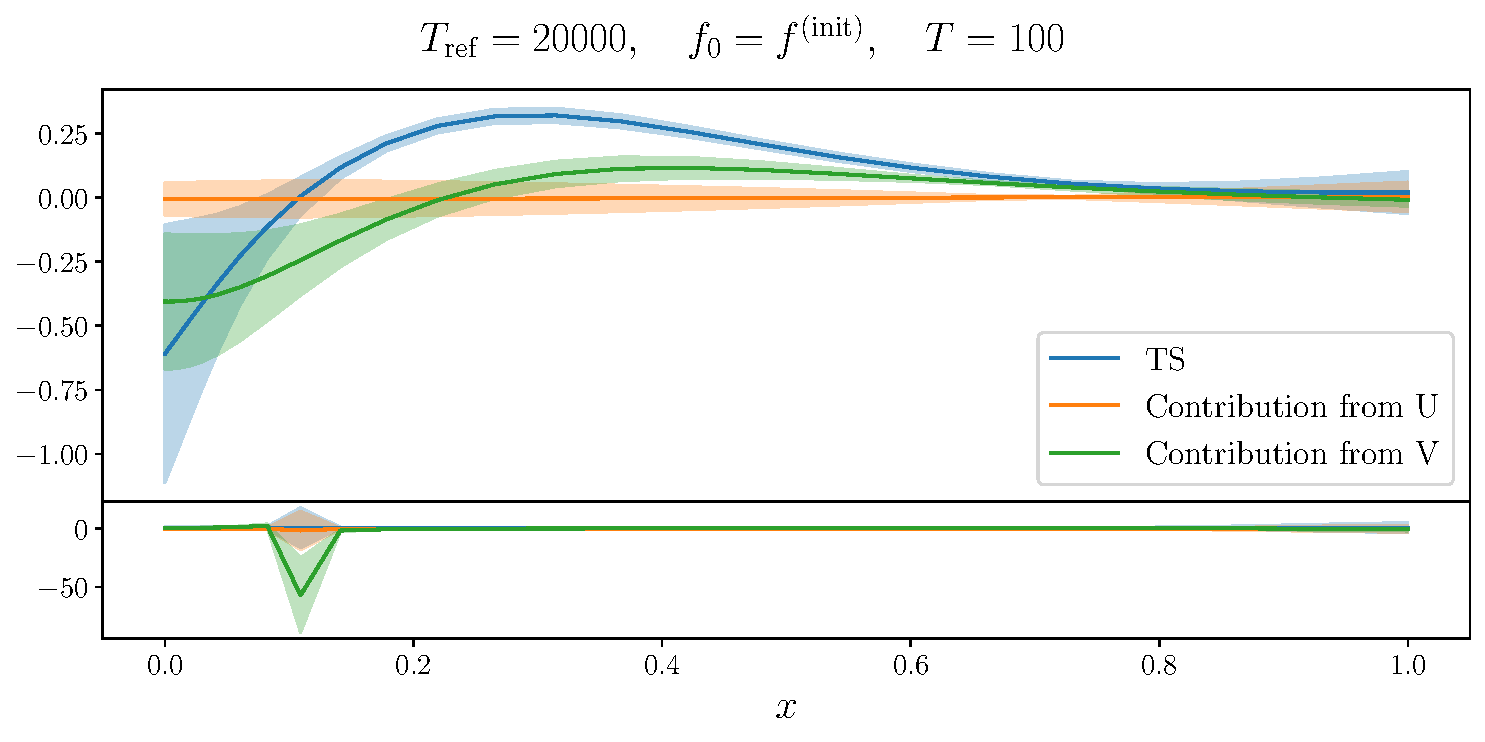
\includegraphics[width=0.45\textwidth]{plots/analytical_solution/pdf_plot_u_v_100_L2.pdf}
    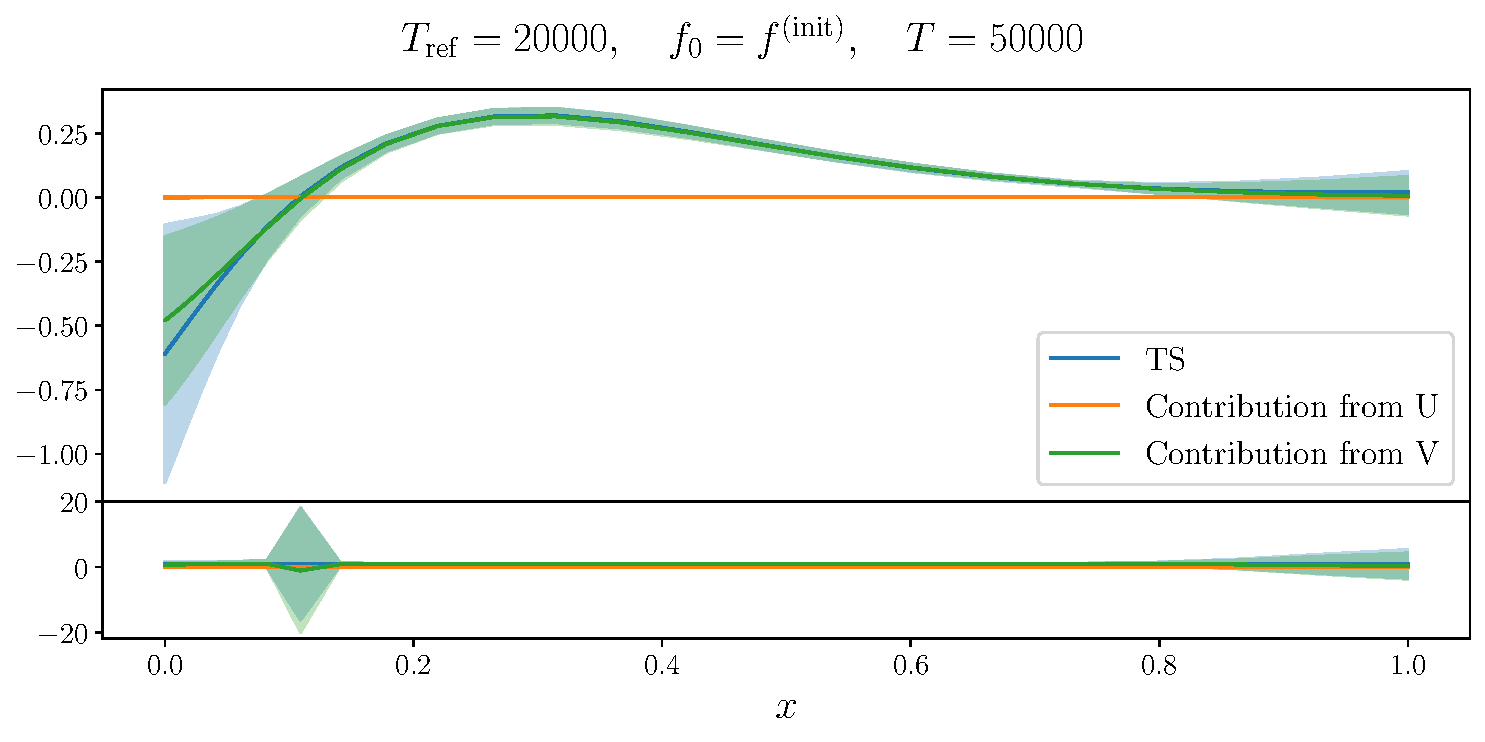
\includegraphics[width=0.45\textwidth]{plots/analytical_solution/pdf_plot_u_v_50000_L2.pdf}
    \caption{Same as Fig.~\ref{fig:xT3_u_v_contributions_L0}, but using L2 data.}
    \label{fig:xT3_u_v_contributions_L2}
  \end{figure}
  % ===================================


\FloatBarrier
